\chapter{Higgs Phenomology}
\label{sec:pheno}

%Dasu -
%The pheno chapter need not start from the Dirac equation and build up. It should have crisp intro to Higgs phenomenology starting from that portion of the Lagrangian. You don’t need all the myriad details of SM like the quark mixing matrices, etc.

In this chapter I provide an increasingly mathematical description of the standard model
of physics, specifically in reference to the Higgs boson. I provide a basic overview of some 
properties of the Higgs boson including how it is created in a hadron collider, an overview
of the possible decay paths for a Higgs boson, and a discussion of the Higgs boson
couplings, or interactions, with different fundamental particles. A description of the
Higgs boson requires covering the process of electroweak symmetry breaking (EWSB) which
provides the mathematical descripition of the process defining the Higgs boson and the
Higgs field.

\section{Standard Model Symmetries}
Many people are attracted to physics because of the beauty they see in the patterns of nature.
PW Anderson, a physics Nobel laureate, stated, ``it is only slightly overstating the case 
to say that physics is the study of symmetry''~\cite{pw_anderson:1972}.
One way of expressing many types of patterns mathematically is with symmetries, properties which 
remain invariant under certain transformations. The SM is defined by a group of symmetries
representing certain conserved properties. Specifically, the SM is represented by  the
symmetries of the unitary product group SU(3)$_{\text{C}} \,\times \,$ SU(2)$_{\text{L}} \, \times\,$ U(1)$_{\text{Y}}$.
These three terms all reflect symmetries and conserved quantities discussed below.

Electric charge ($Q$), the third component of weak isospin ($T_{3}$), and hypercharge ($Y$) act together to define a conserved 
quantity in the SM, $Q = T_{3} + \frac{Y}{2}$. This is represented by the
hypercharge U(1)$_{\text{Y}}$ symmetry group.

The two SU($n$) groups are special unitary groups which represent rotations.
In the SM, the SU(2) group provides a description of particle spin.
The ``L'' subscript for the SU(2)$_{\text{L}}$ group indicates that that it only couples to
and describest left handed fermions.
The SU(3)$_{\text{C}}$ group describes the local symmetry of color charge.


\section{Electroweak Symmetry Breaking}
Glashow, Weinberg, and Salam demonstrated a unified description of the electromagnetic force 
and weak force which merge at energies of order 100\GeV into the electroweak force,
described by the electroweak Lagrangian~\cite{Glashow:1961tr,SM1,SM3}.
The electroweak Lagrangian defines a gauge field theory which is 
invariant under the SU(2)$_{\text{L}} \, \times \, $U(1)$_{\text{Y}}$ symmetry group. 
Prior to the introduction of Electroweak Symmetry Breaking (EWSB),
the electroweak Lagrangian describes massless $\PW$ and $\PZ$ bosons.
However, as previously mentioned, the $\PW$ and $\PZ$ bosons were discovered in 1983
and found to be two of the most massive particles~\cite{AUBERT1983275,1983398}. 
EWSB rescues what would be a collasal disagreement between theoretical prediction
and experimental results. The introduction of EWSB to the theory preserves the structure of
the electroweak interactions and succeedes in endowing the $\PW$ and $\PZ$ bosons
with mass.

Electroweak symmetry breaking is an application of spontaneous symmetry breaking to
the electroweak Lagrangian. It is achieved via the Brout--Englert--Higgs
mechanism~\cite{Englert:1964et,Higgs:1964ia,Higgs:1964pj,Guralnik:1964eu,Higgs:1966ev,Kibble:1967sv},
leading, in its minimal version, to the prediction of the existence of one physical neutral scalar particle,
commonly known as the Higgs boson. The EWSB mechanism, defined by Brout, Englert, and Higgs,
proposes a self-interacting complex doublet scalar field,
\begin{equation}
\phi = \Bigg(\frac{\phi_{\alpha}}{\phi_{\beta}}\Bigg) = 
    \sqrt{\frac{1}{2}} \Bigg(\frac{\phi_{1} + i\phi_{1}}{\phi_{3} + i\phi_{4}}\Bigg),
\label{eqn:phi_doublet}
\end{equation}

that is applied to the electroweak Lagrangian, 
\begin{equation}
\mathcal{L} = \big(D_{\mu}\phi\big)^{\dagger} \big(D^{\mu}\phi\big) - V\big(\phi\big),
\end{equation}

where $D^{\mu}$ is the covariant derivative and the potential, $V\big(\phi\big)$, 
is expressly defined with two terms, 
\begin{equation}
V\big(\phi\big) = \mu^{2}\phi^{\dagger}\phi + \lambda\big(\phi^{\dagger}\phi\big)^{2}
\label{eqn:v_pot}
\end{equation}

The Lagrangian describes a system of four scalar particles, the $\phi_{i}$,
of equation~\ref{eqn:phi_doublet} each with mass $\mu$. 
To achieve EWSB, the constants in the potential $V\big(\phi\big)$ are defined such that $\mu^{2} < 0$
and $\lambda > 0$. The choice $\mu^{2} < 0$ and $\lambda > 0$ lead to a potential $V\left(\phi\right)$
similar to what is shown in Figure~\ref{fig:higgs_potential}. Expanding around a choosen minima of the potential
$V\big(\phi\big)$, $v$, and taking $\phi_{1} = \phi_{2} = \phi_{4} = 0$ and
$\phi_{3}^{2} = -\frac{\mu^{2}}{\lambda} \equiv v^{2}$, $\phi$ becomes
\begin{equation}
\phi = \sqrt{\frac{1}{2}} \Bigg(\frac{0}{v}\Bigg),
\label{eqn:phi_doublet_exp}
\end{equation}

where the scalar doublet, $\phi$ acquires a non-zero vacuum expectation value (VEV), $v \approx 246\GeV$.
In this process a neutral and two charged massless Goldstone bosons~\cite{PhysRev.127.965} are generated. These Goldstone
bosons mix with the fields corresponding to the broken SU(2)$_{\text{L}} \,\times\,$ U(1)$_{\text{Y}}$
symmetries giving masses to the $\PW$ and $\PZ$ bosons. The single remaining component of the
original complex doublet $\phi$ becomes a new fundamental scalar particle 
known as the Higgs boson with a mass
\begin{equation}
\mH^{2} = 2\lambda v^2
\end{equation}

%Applying EWSB to the SM takes the symmetries expressed as 
%SU(3)$_{\text{C}} \,\times \,$ SU(2)$_{\text{L}} \,\times \,$ U(1)$_{\text{Y}}$ and turns them into
%SU(3)$_{\text{C}} \, \times \,$ U(1)$_{\text{em}}$.

\begin{figure*}[htbp]
\centering
     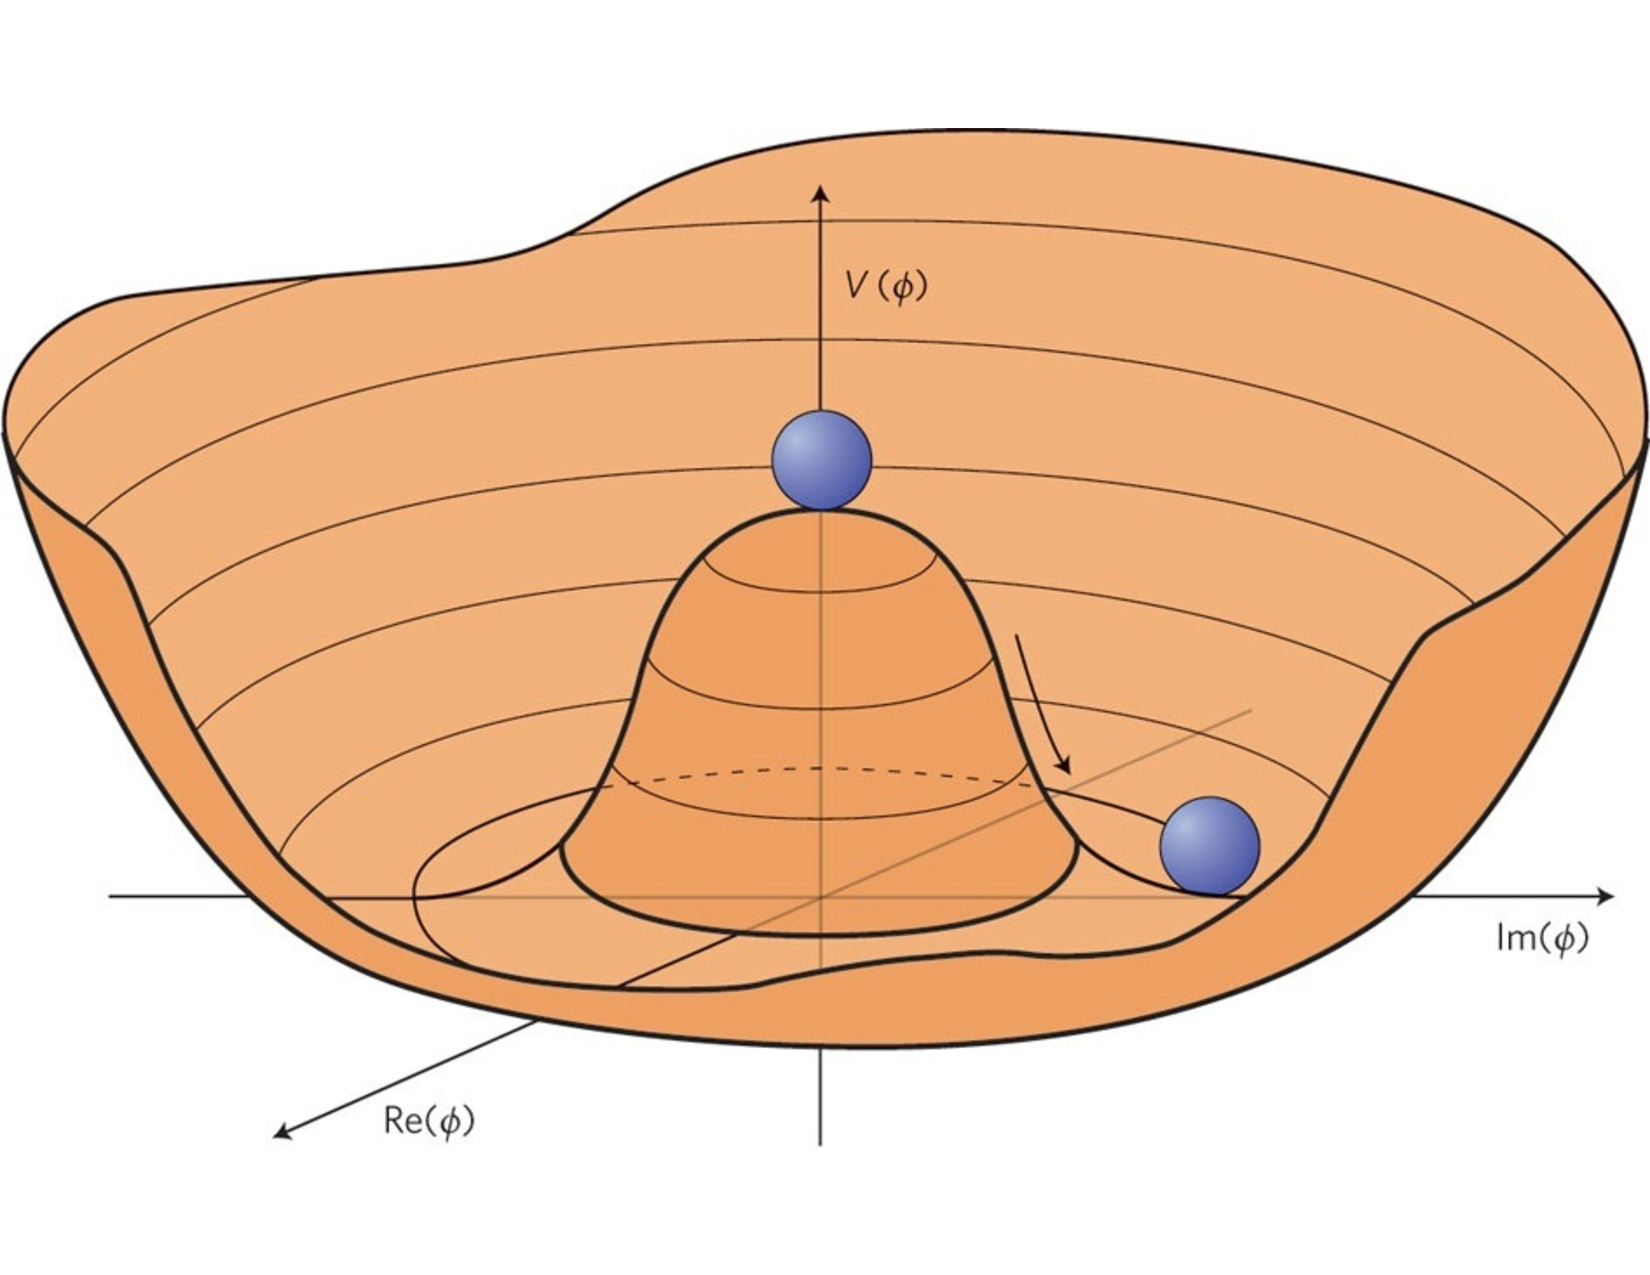
\includegraphics[width=0.55\textwidth]{phenomology_of_processes/plots/higgs_potential.pdf}
     \caption{
The potential $V\left(\phi\right)$ from Equation~\ref{eqn:v_pot} showing a non-stable state
at the origin and a stable state in the circular trough.
     }
     \label{fig:higgs_potential}
\end{figure*}



\section{Higgs Yukawa Couplings}
In addition to providing a mechanism for the $\PW$ and $\PZ$ bosons to gain mass in the SM, EWSB also
provides a mechanism for the fermions to acquire mass through their interactions with the Higgs boson
via Yukawa couplings. A Yukawa coupling is an interaction between a scalar field and a Dirac field
similar to,
\begin{equation}
V \approx h_{f}\bar{\psi_{f}}\phi\psi_{f},
\end{equation}

where the Dirac fields, $\psi$, describe fermions and the scalar field, $\phi$, is taken to be that of the Higgs boson. 
The introduction of a Yukawa interaction linking together the fermions and the Higgs boson,
results in massive fermions where their mass can be written as,
\begin{equation}
m_{f} = \frac{h_{f} v}{\sqrt{2}}
\label{eqn:yukawa_c}
\end{equation}

which covers the masses for the nine charged fermions: the three charged leptons and six quarks.
The EWSB mechanism nor the Yukawa interaction provide insight into the larger variety of fermion
masses. Instead, the fermion masses are taken as free parameters of the SM and the values
$h_{f}$ represent the Yukawa coupling parameter for each of the fermions.

The mass of nine charged fermions are known experimentally, most to very high precision.
The $\Pgt$ lepton is known to be $1776.82\pm0.16\MeV$~\cite{PDG}.
Knowing this, the $\Pgt$ lepton to Higgs boson Yukawa coupling can be calculated from theory
and compared against experimental results. 

Exploring the Higgs boson to fermions decay process is the most promissing way to directly probe
the Higgs boson Yukawa couplings. The Higgs boson decay process are discussed below in 
Section~\ref{sec:higgs_decays} where this discussion continues.

%with equation~\ref{eqn:yukawa_c},
%\begin{equation}
%h_{\Pgt} = \frac{\sqrt{2} \, m_{\Pgt}}{v} = \sqrt{2}\frac{1.78\GeV}{246\GeV} = 0.0102
%\label{eqn:yukawa_tau}
%\end{equation}



\section{Higgs Production}
The Higgs boson is produced according to it couplings and interactions in the SM
Lagrangian. Understanding the different production mechanisms for the Higgs boson
allows experimentalists to search for unique signatures in collisions to better
help separate the Higgs boson process from the many other interactions.
At a hadron collider like the LHC, the Higgs boson production
mechanisms begin from initial states of quarks and gluons. The Higgs boson
only couples to massive particles eliminating direct gluon to Higgs boson processes
as is seen in Figure~\ref{fig:sm_forces} from the introduction.
However, the largest Higgs boson production process at the LHC begins with a gluon
initial state and is called gluon fusion and is discussed below.

Feynman diagrams of the leading Higgs boson production processes for
proton-proton collsisions, at the LHC, when operating at 13\TeV center-of-mass energy,
are shown in Figure~\ref{fig:higgs_feyn}. 
The cross sections for the leading Higgs boson production processes
are shown in Figure~\ref{fig:higgs_production}. The values for the leading
processes are approximately: $ggH \approx 49\pb$, VBF$ \approx 3.8\pb$, $\PW\PH \approx 1.4\pb$,
and $\PZ\PH \approx 0.88\pb$~\cite{deFlorian:2016spz}. The $\ttbar\PH$ process,
which is found to be relatively insignificant in the following analyses, has a cross
section approximatly half the size of the next smallest one, $\PZ\PH$, where
$\ttbar\PH \approx 0.51\pb$.


\begin{figure*}[htbp]
\centering
     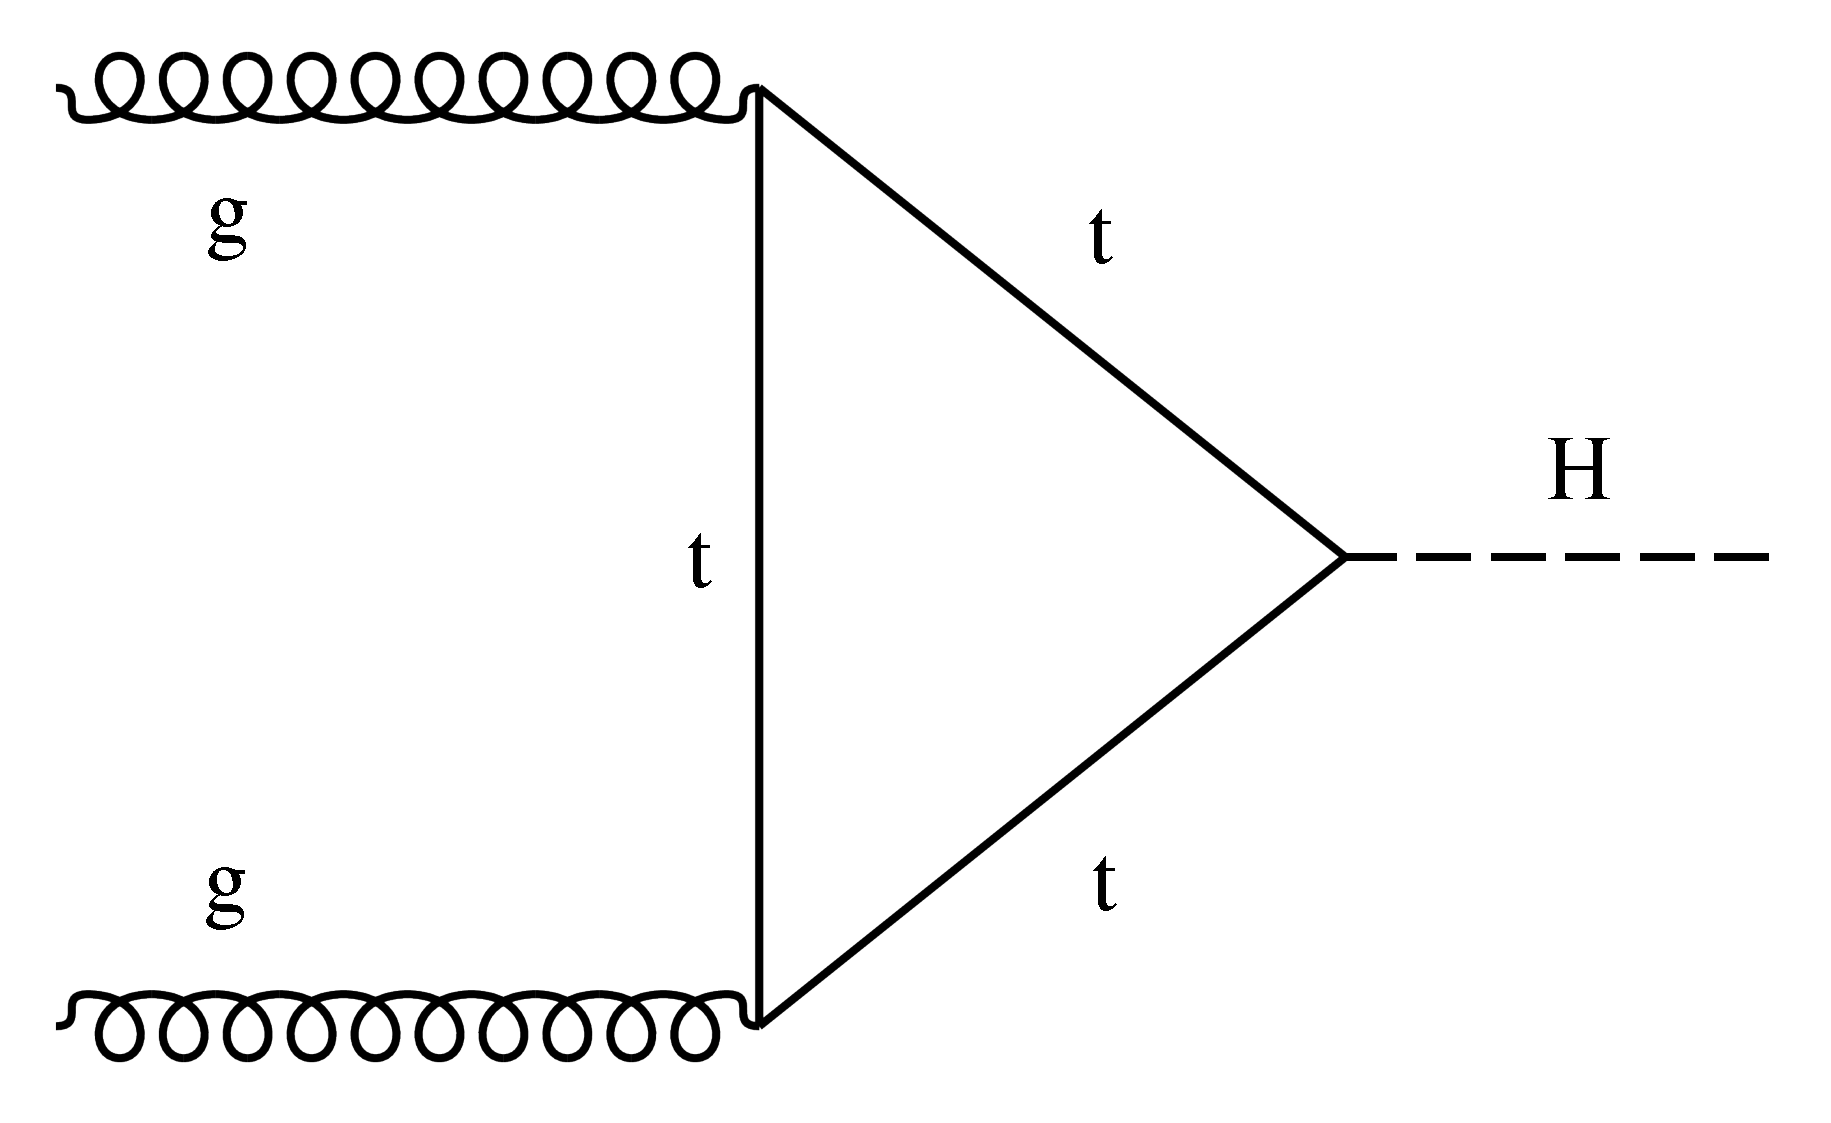
\includegraphics[width=0.35\textwidth]{phenomology_of_processes/plots/feyn_ggH.pdf}
     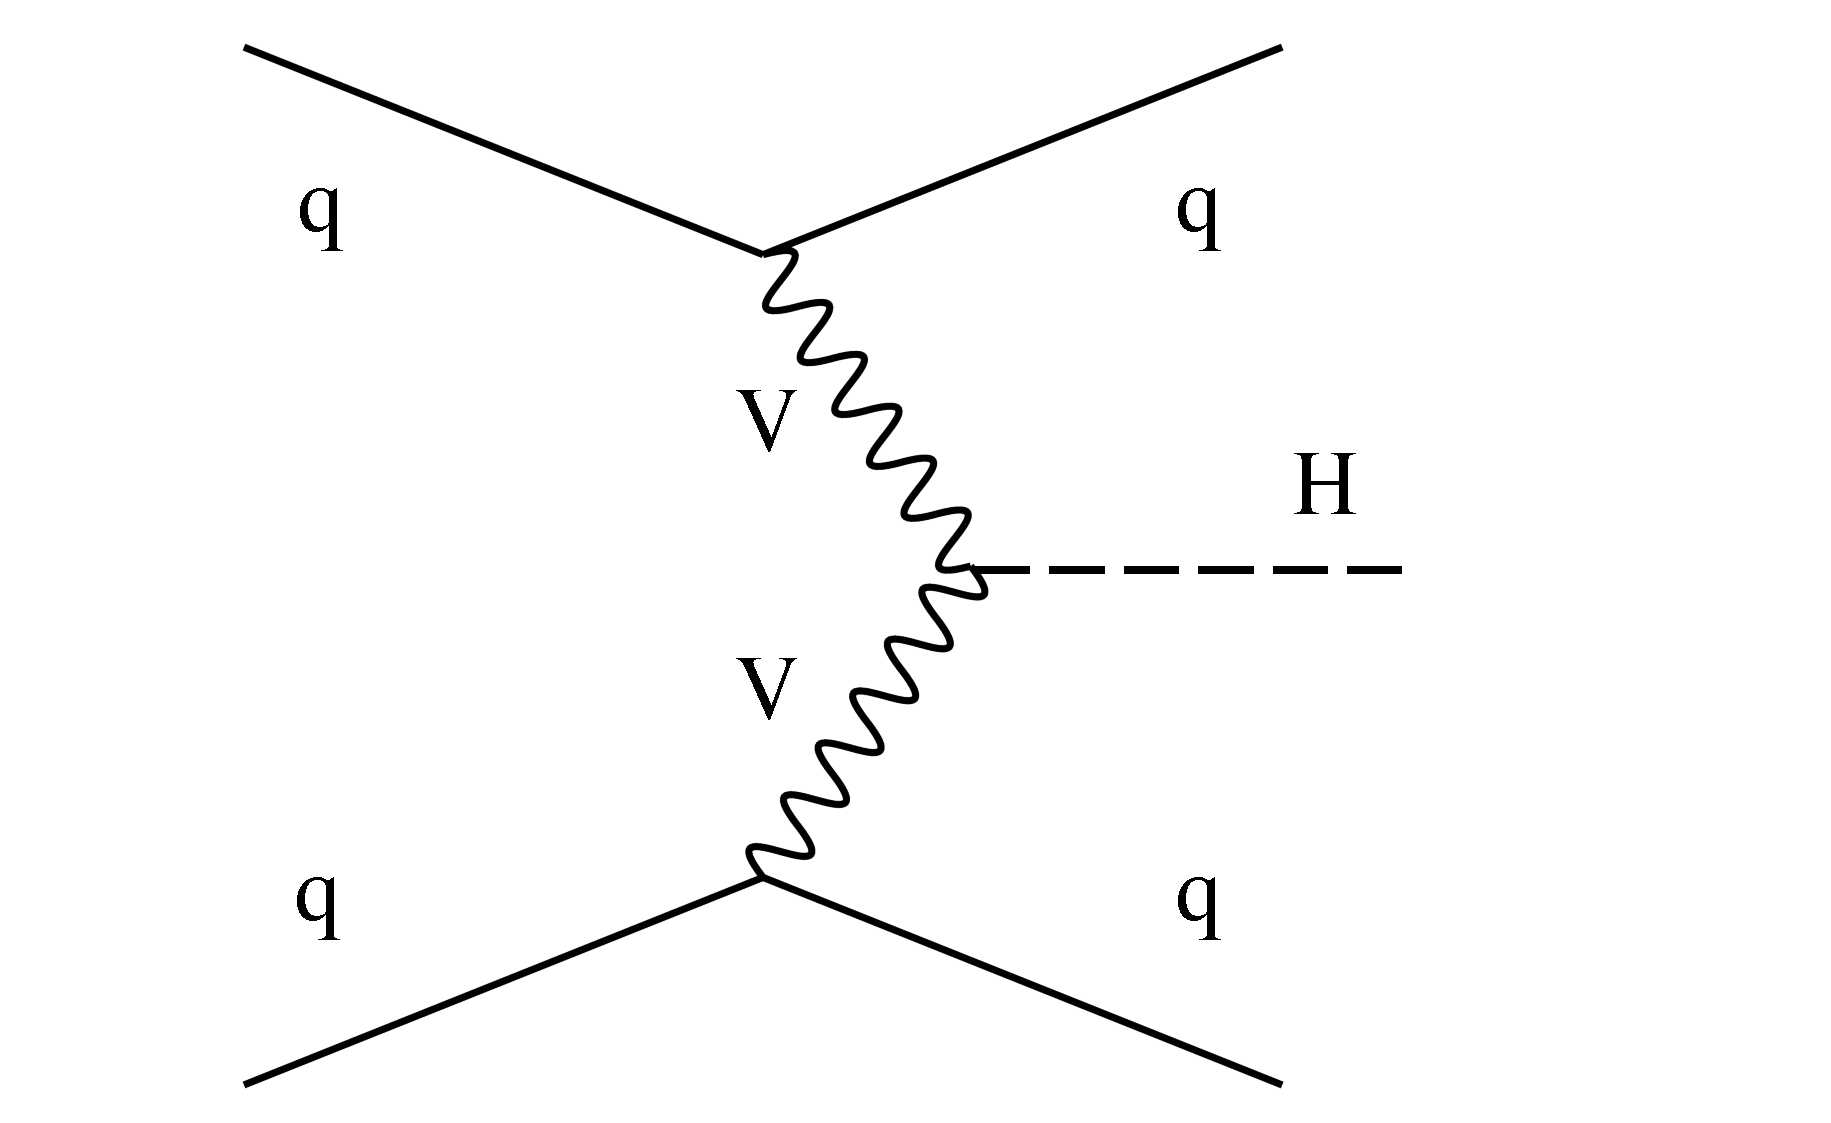
\includegraphics[width=0.35\textwidth]{phenomology_of_processes/plots/feyn_qqH.pdf}
     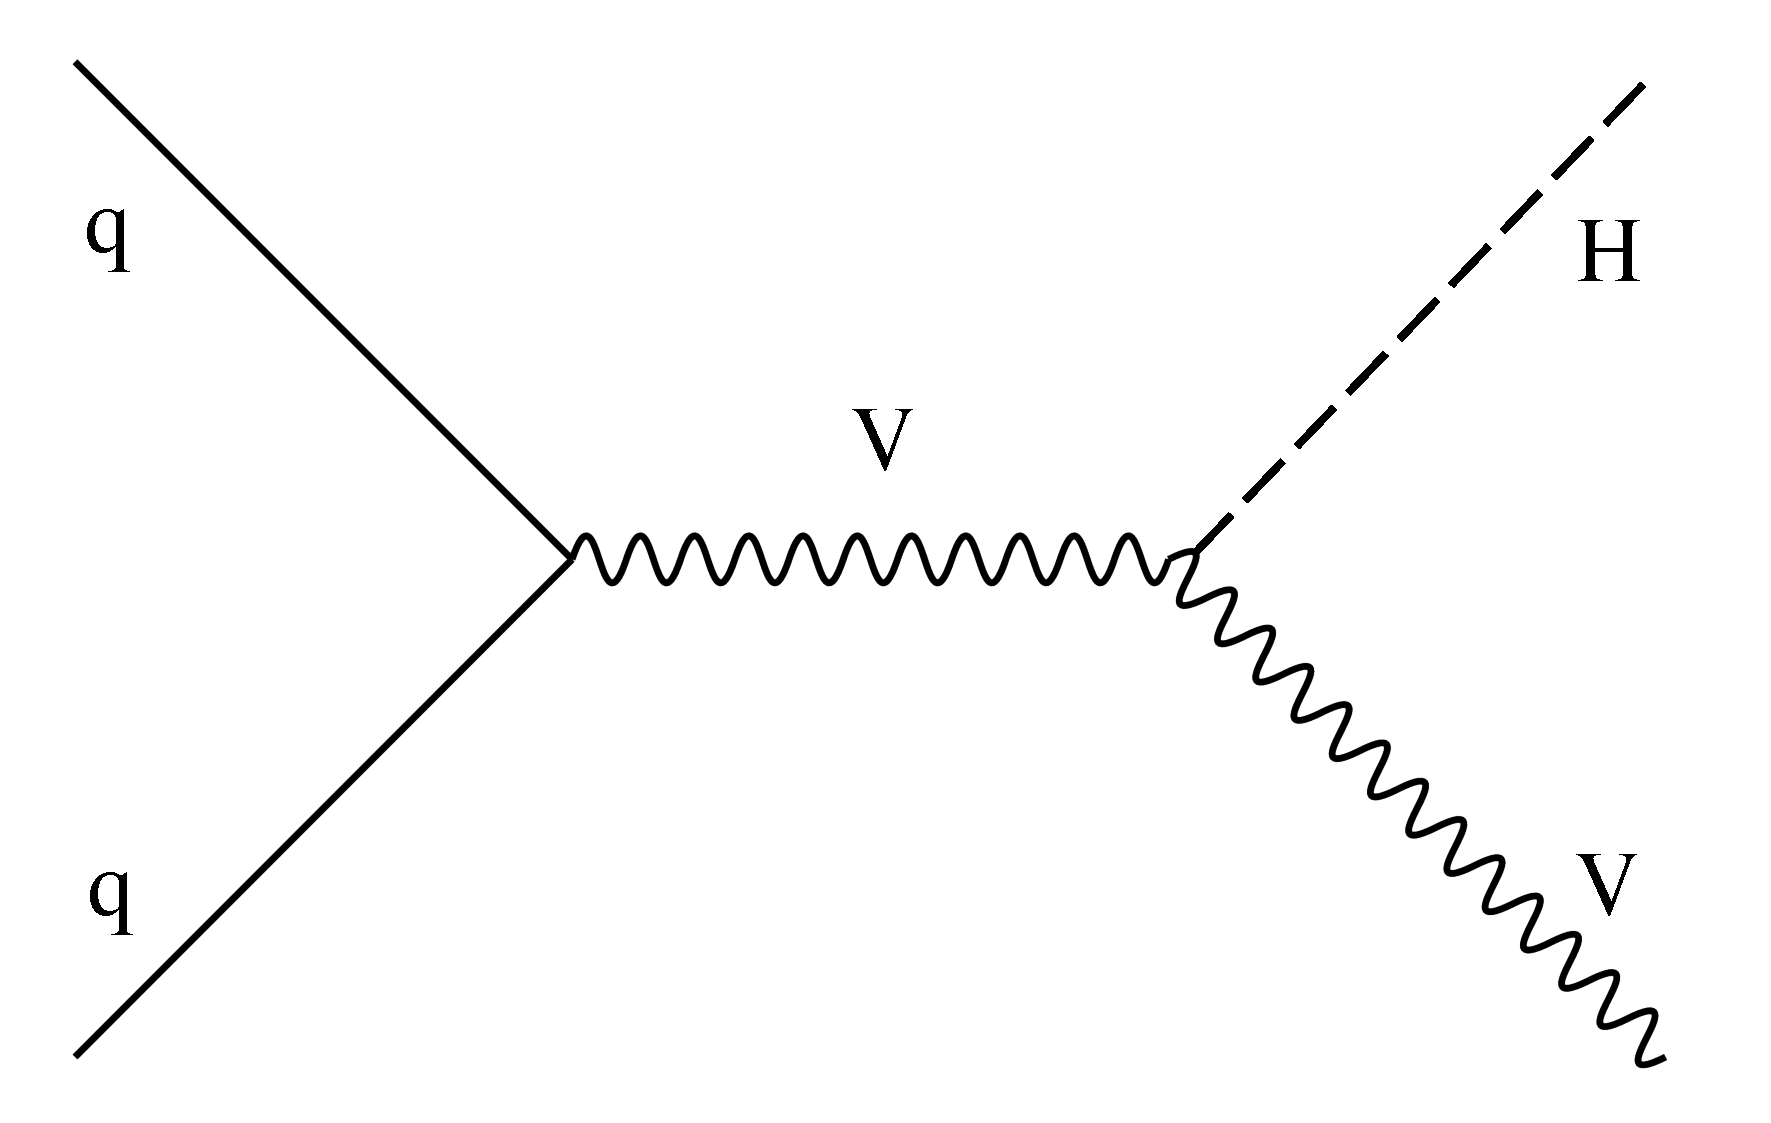
\includegraphics[width=0.35\textwidth]{phenomology_of_processes/plots/feyn_VH.pdf}
     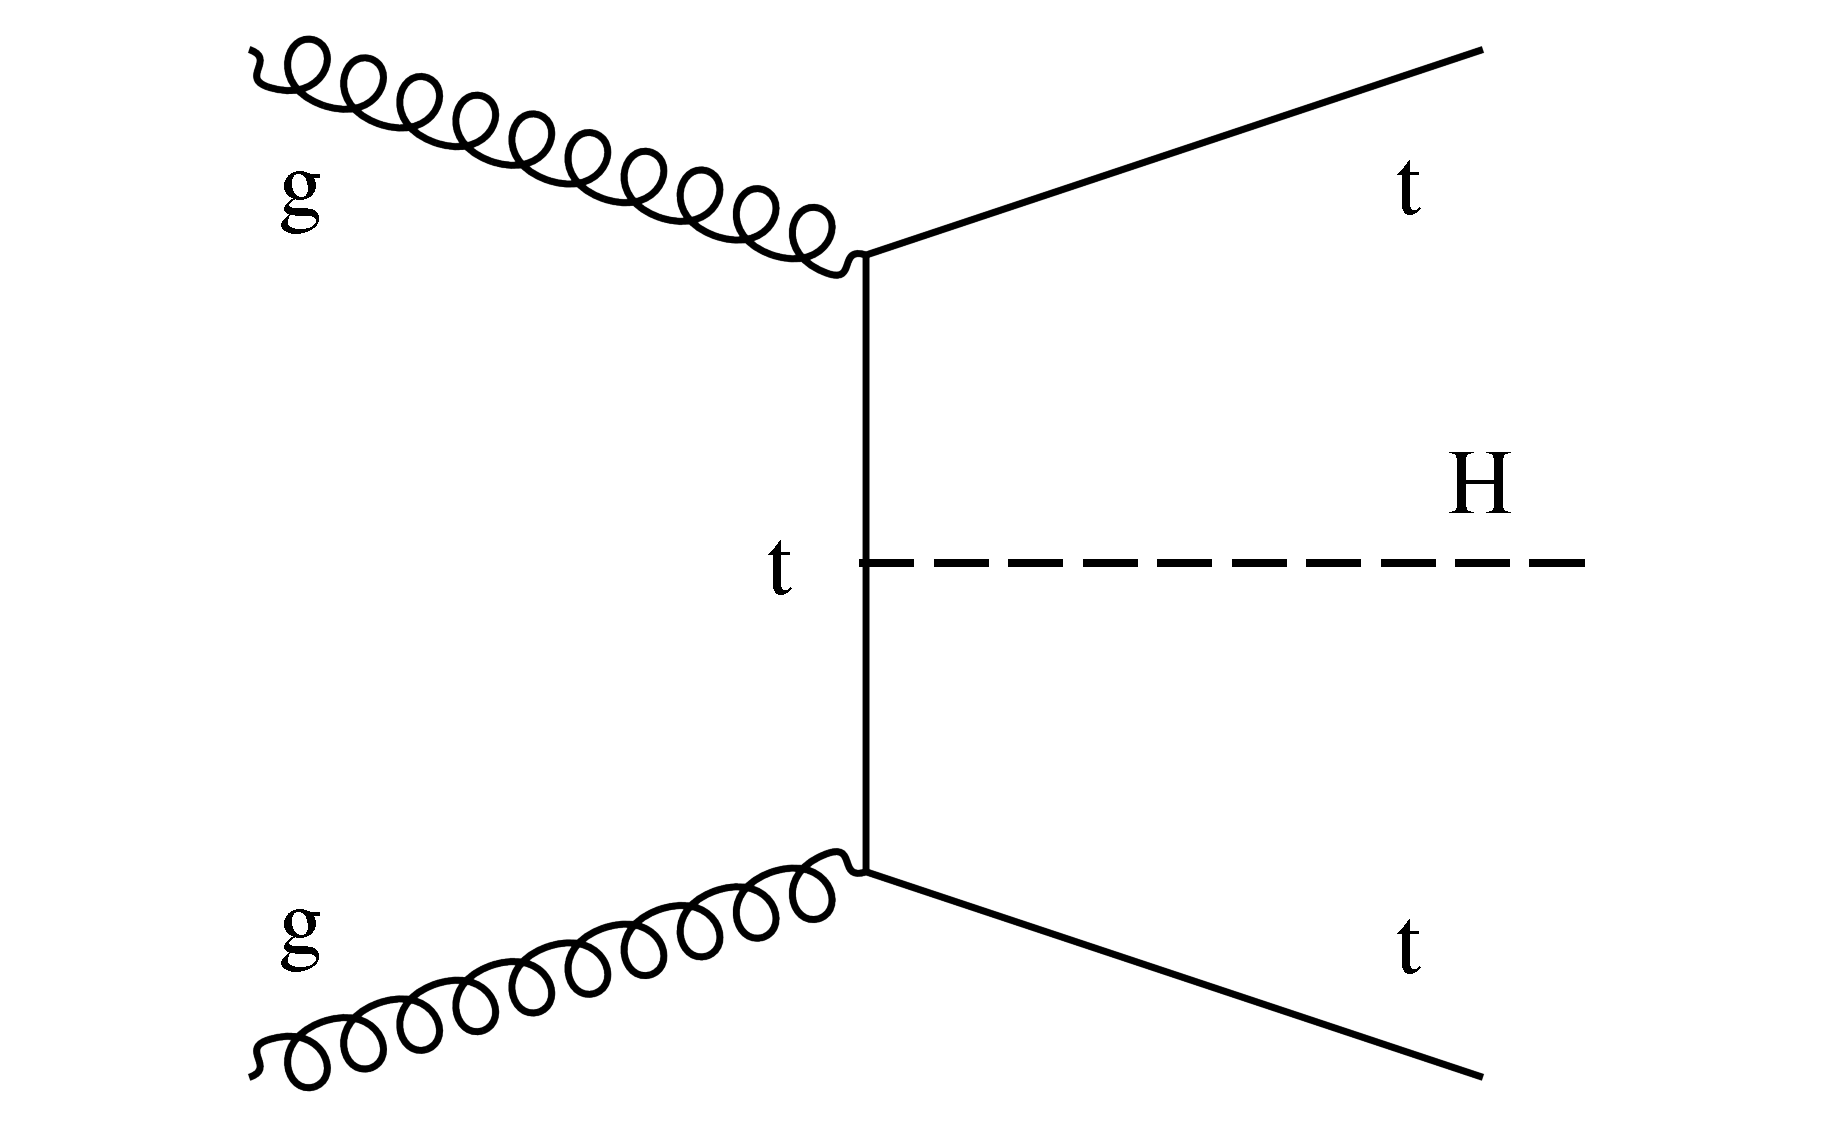
\includegraphics[width=0.35\textwidth]{phenomology_of_processes/plots/feyn_ttH.pdf}
     \caption{
Feynman diagrams representing the leading Higgs boson production processes.
Progressing in order of largest to smallest of these production cross sections:
(top left) gluon fusion, (top right) vector boson fusion, (bottom left)
associated production covering both the $\PW\PH$ and $\PZ\PH$ processes,
and (bottom right) top-quark associated production.
     }
     \label{fig:higgs_feyn}
\end{figure*}


\begin{figure*}[htbp]
\centering
     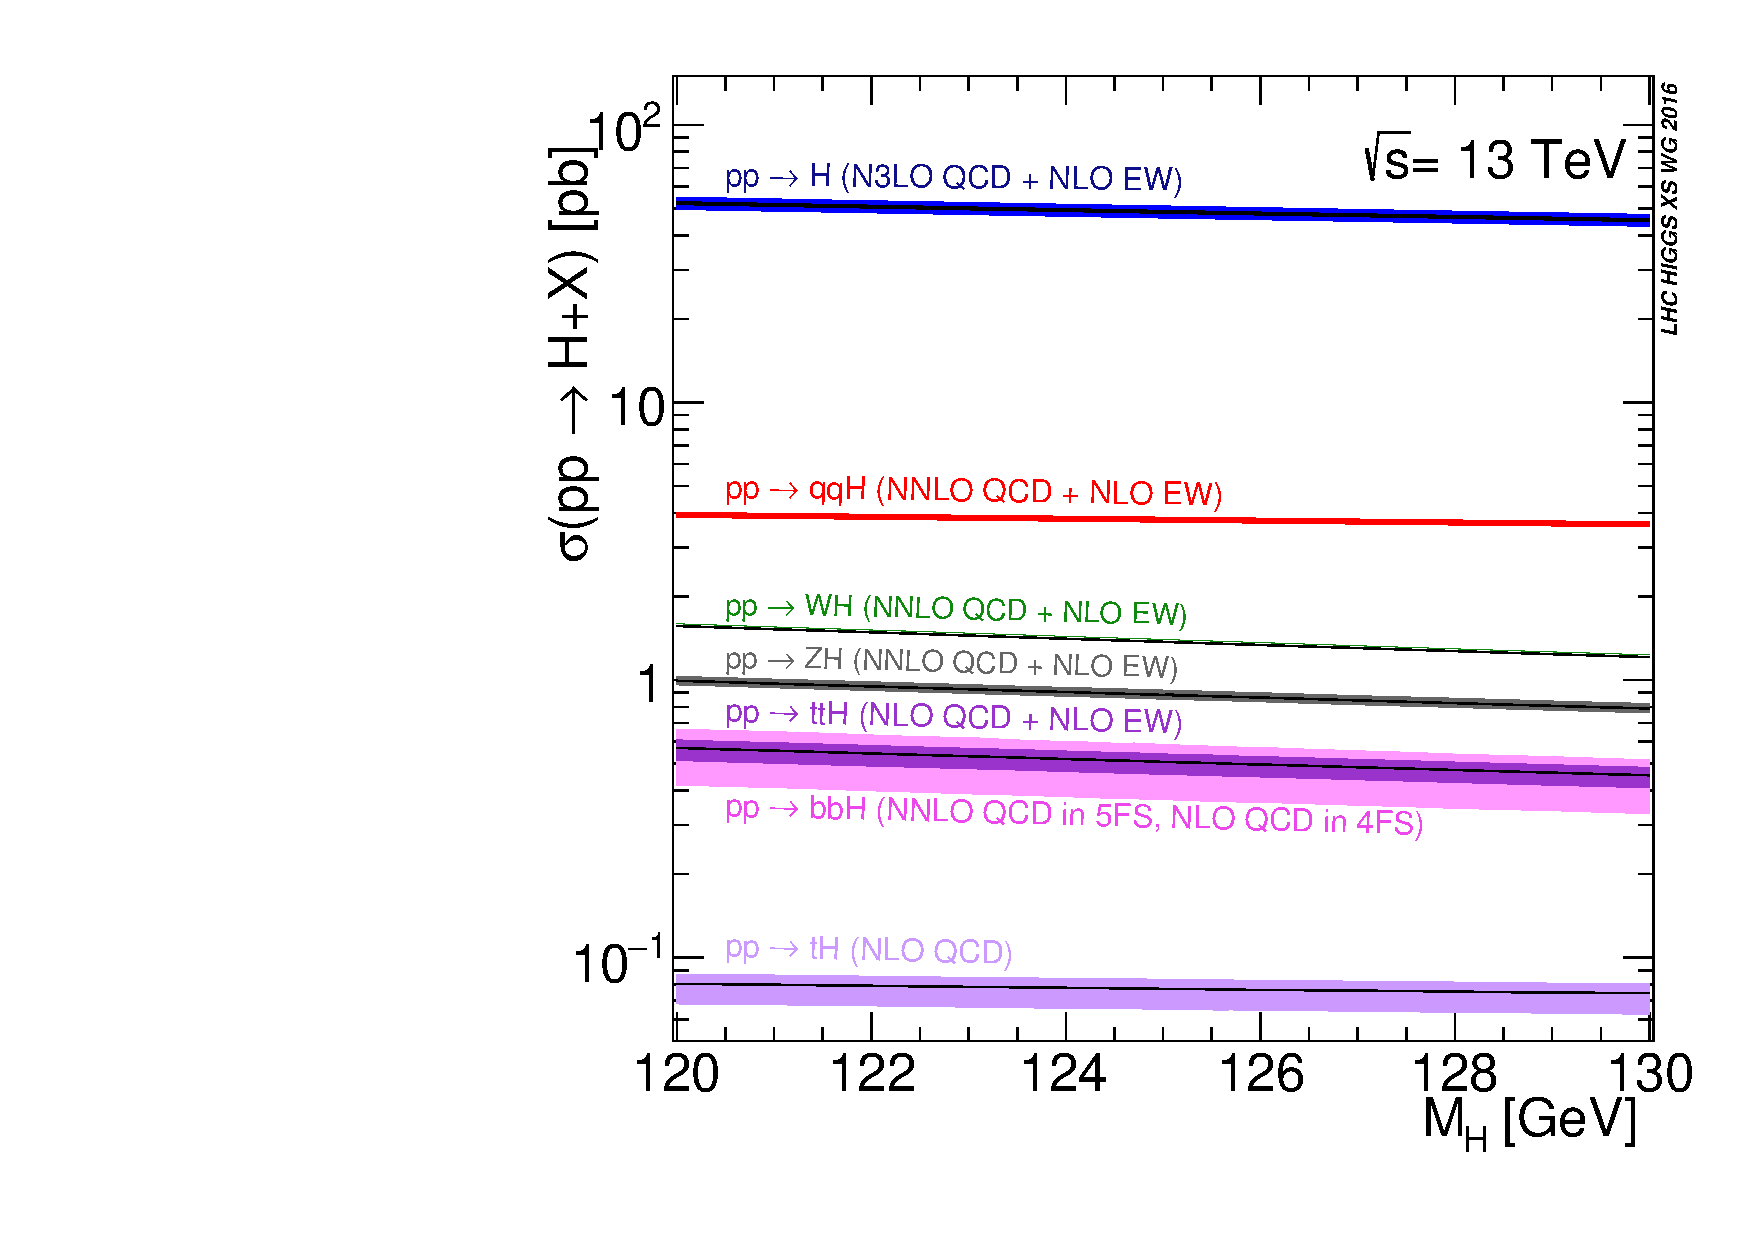
\includegraphics[width=0.65\textwidth]{phenomology_of_processes/plots/plot_13tev_H_sqrt.pdf}
     \caption{
The theorized Higgs boson production cross sections and their uncertainties,
as a function of the Higgs boson mass, are shown. The gluon fusion process ($ggH$)
is denoted as pp $\to$ H in the figure.
The CMS and ATLAS experiments have determined $\mH = 125.09\GeV$~\cite{Aad:2015zhl}.
     }
     \label{fig:higgs_production}
\end{figure*}


\subsection{Gluon Fusion}
$ggH$ - mediated by the exchange of a virtual, heavy top quark, Contributions from lighter quarks propagating in the loop are suppressed proportional to $m^{2}_{q}$.
To a very good approximation, the leading top-quark contribution can be evaluated in the limit $m_{t} \to \inf$ [24,25].

\subsection{Vector Boson Fusion}
Higgs production via VBF, qq → qqH, proceeds by the scattering of two (anti-)quarks, mediated by t- or u-channel exchange of a W or Z boson, with the Higgs boson radiated off the weak-boson propagator. The scattered quarks give rise to two hard jets in the forward and backward regions of the detector. Because of the color-singlet nature of the weak-gauge boson exchange, gluon radiation from the central-rapidity regions is strongly suppressed. These characteristic features of VBF processes can be exploited to distinguish them from overwhelming QCD backgrounds, including gluon-fusion induced Higgs + 2 jet production, and from s-channel WH or ZH production with a hadronically decaying weak gauge boson. After the application of specific selection cuts, the VBF channel provides a particularly clean environment, not only for Higgs searches but also for the determination of Higgs boson couplings at the LHC [74].

\subsection{Associated Production}

\section{Higgs Decays}
\label{sec:higgs_decays}

After a Higgs boson is produced, it will decay extremly rapidly. The theorized lifetime of a Higgs
boson particle is $1.6 \times 10^{-22}$ s~\cite{Dittmaier:2012vm} meaning that, when created
inside of the CMS detector, a Higgs boson will always decay
within the CMS detector . There are multiple possible decay
paths each with their own probability or branching ratio with the largest branching ratio
processes shown in Figure~\ref{fig:higgs_decay}. The $\htt$ process has a branching
ratio of approximately 6.3\% for $\mH = 125\GeV$.


\begin{figure*}[htbp]
\centering
     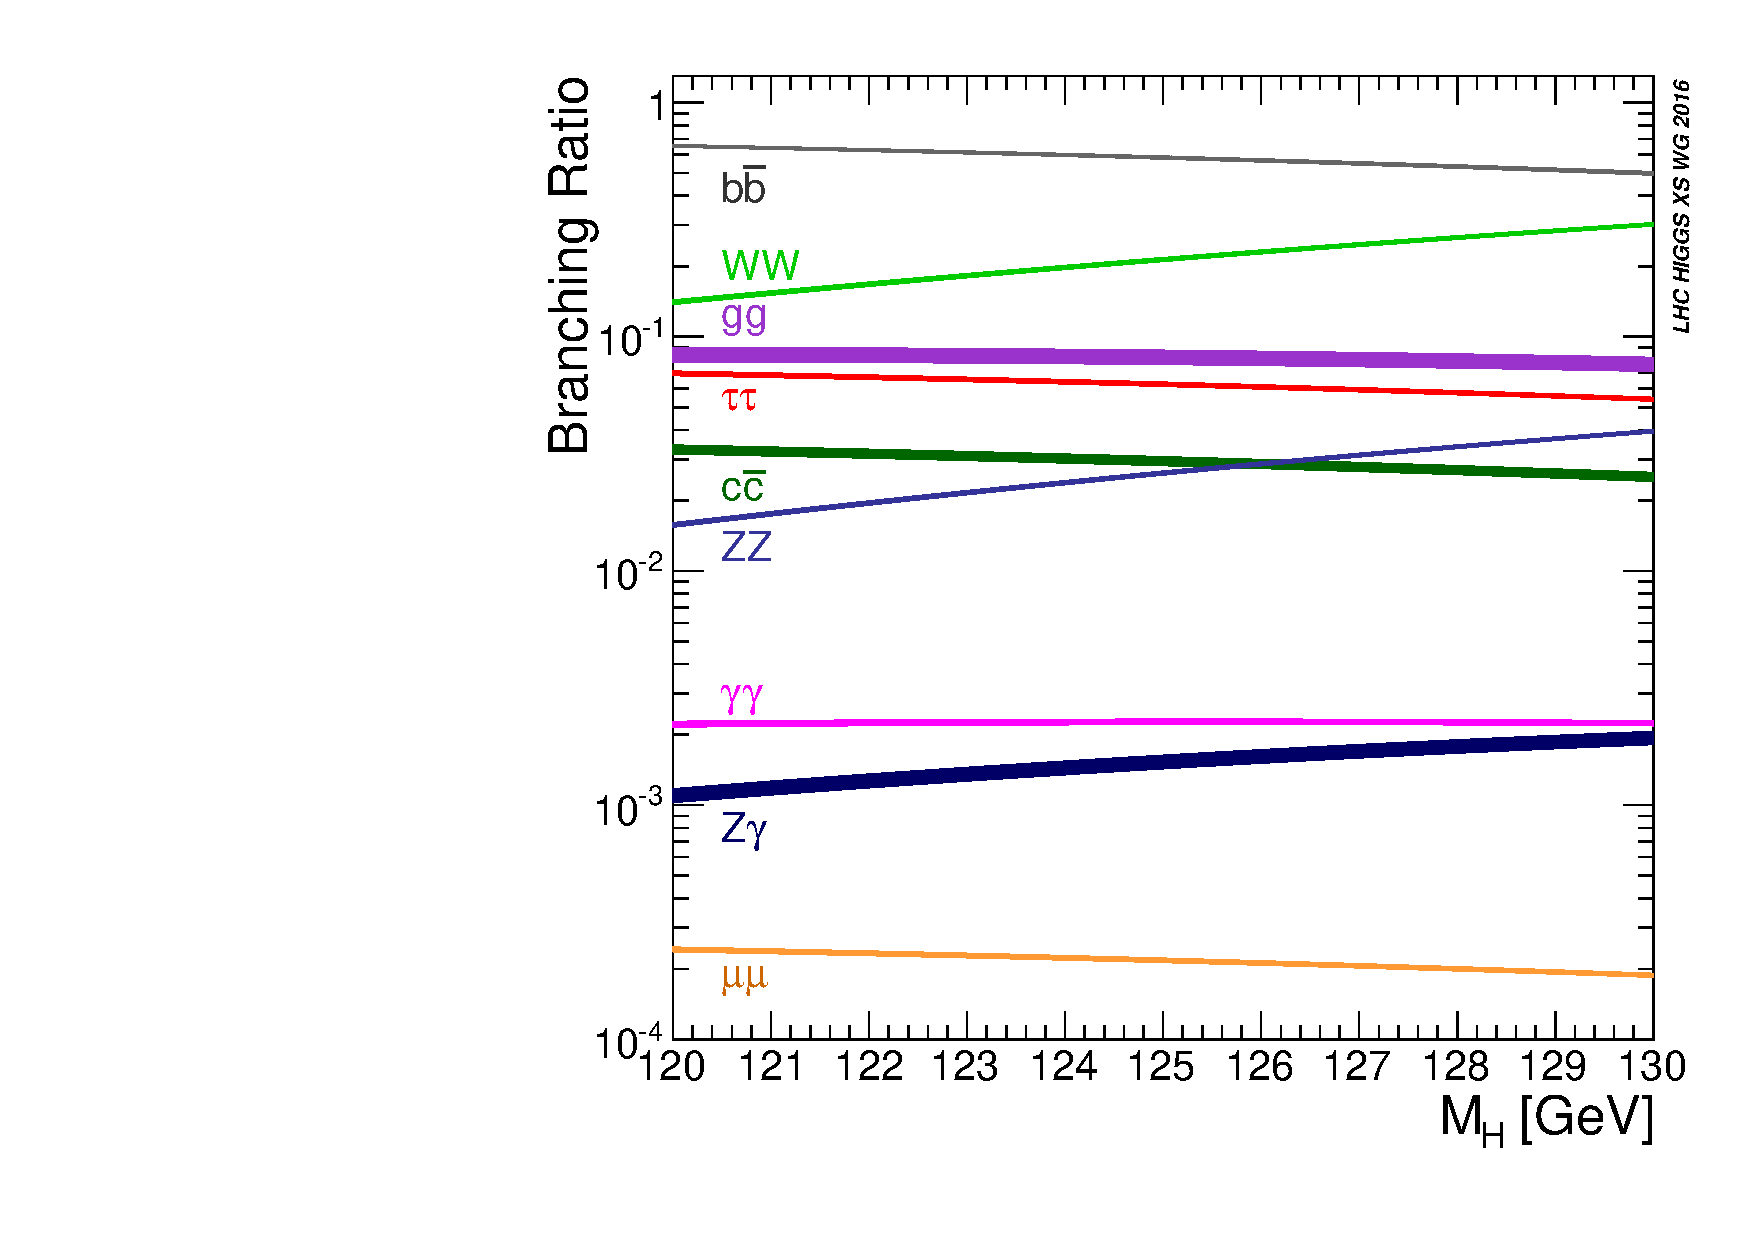
\includegraphics[width=0.65\textwidth]{phenomology_of_processes/plots/SMHiggsBR_YR4-square.pdf}
     \caption{
The different theorized Higgs boson decay process are shown as a 
as a function of the Higgs boson mass.
The CMS and ATLAS experiments have determined $\mH = 125.09\GeV$~\cite{Aad:2015zhl}.
     }
     \label{fig:higgs_decay}
\end{figure*}


To establish the mass generation mechanism for fermions,
 it is necessary to probe the direct coupling of
the Higgs boson to such particles.
The most promising decay channel is $\Pgt^+\Pgt^-$,
because of the large event rate expected in the SM compared to the $\Pgm^+\Pgm^-$ decay channel ($\mathcal{B}(\PH\to\Pgt^+\Pgt^-)=6.3$\% for a mass of 125.09\GeV), and of the smaller contribution from background events
with respect to the $\bbbar$ decay channel.

\subsection{Higgs to $\tau\tau$ Decay Process}

Estimated as 6.3\% with a relative theoretical uncertainty of $\pm5.7\%$~\cite{deFlorian:2016spz}.




The various production cross sections and branching fractions for the SM Higgs 
boson production, and their corresponding uncertainties are taken from 
References.~\cite{deFlorian:2016spz,Denner:2011mq,Ball:2011mu} and references therein.




%\subsection{QCD and Proton Structure}









